\chapter{Related work}\label{chap3}

\section{Brick}
Brick is a uniform metadata schema designed to represent building
entities—such as equipment, sensors, and spatial locations—and the
relationships between them using an ontology-based framework~\cite{Balaji2016Brick}.
The project was initiated by a consortium of U.S. and European
universities and research institutes, including UC Berkeley, UCLA,
Carnegie Mellon University, UC San Diego, University of Virginia,
University of Southern Denmark, and IBM Research Ireland.
The work was first presented at ACM BuildSys 2016 and continues
to evolve under the open-source Brick Schema community
(\url{https://brickschema.org}).


It addresses the interoperability challenges of heterogeneous Building
Management Systems (BMS), where vendor-specific naming and label
inconsistencies hinder the portability of applications. Brick defines a
normalized vocabulary (tags and tag sets) along with fundamental
relationships like \emph{hasPoint}, \emph{isPartOf}, \emph{feeds}, and
\emph{controls}, enabling semantic queries over RDF-based knowledge
graphs via SPARQL.

\begin{figure}[ht!]
    \centering
    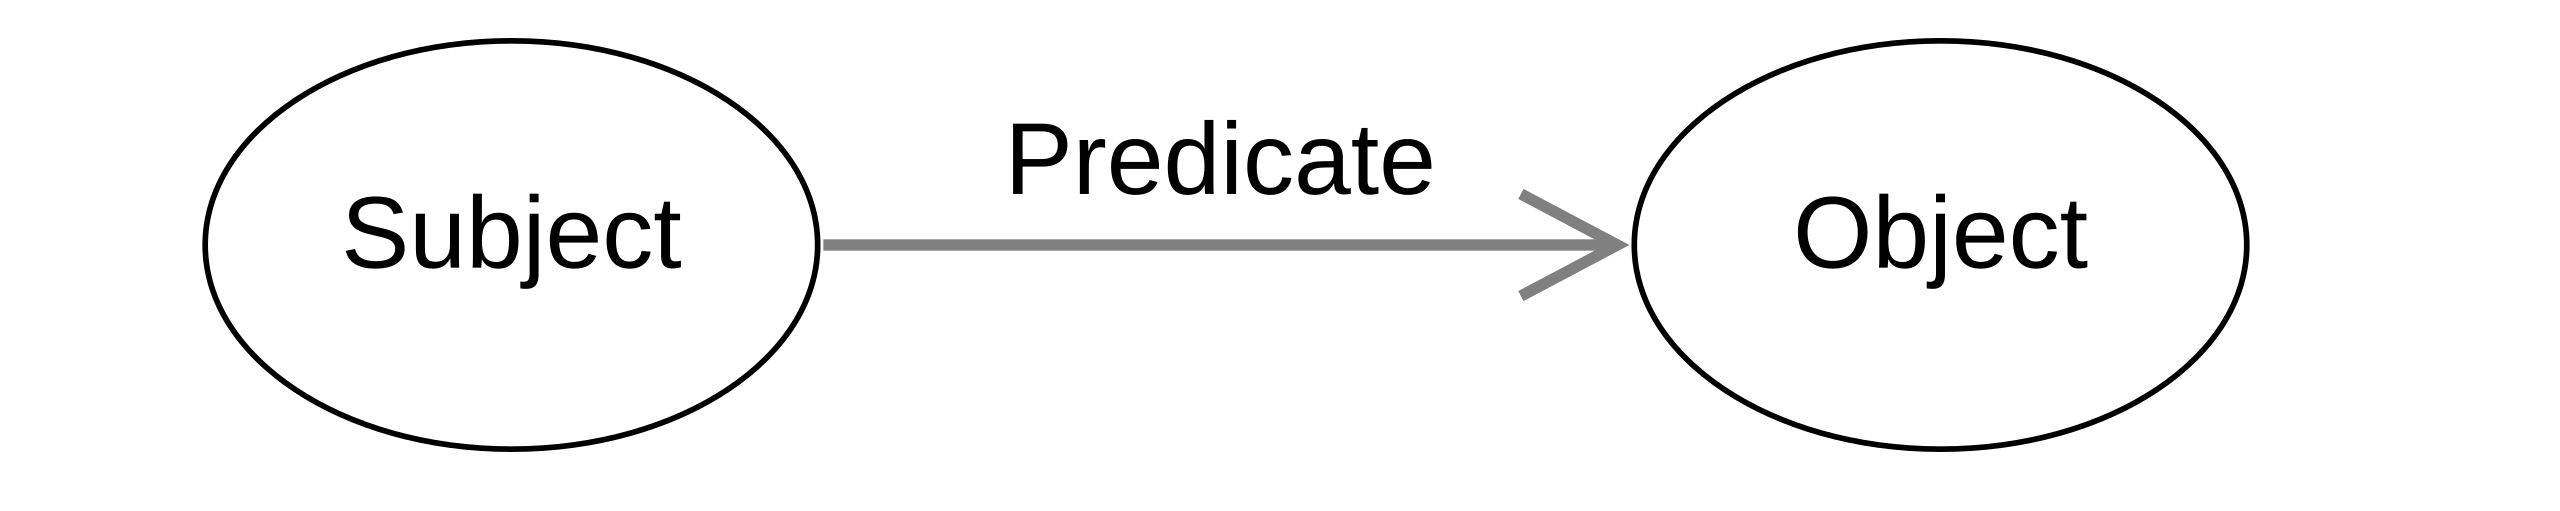
\includegraphics[width=0.7\textwidth]{Images/Basic_RDF_Graph.svg}
    \caption{\textbf{An RDF graph with triple connecting}
    }
    \label{fig:RDF}
\end{figure}

A key design choice of Brick is its reliance on the Resource
Description Framework (RDF). RDF is a W3C standard data model for
representing information as a graph of triples, each consisting of a
\emph{subject}, \emph{predicate}, and \emph{object}. For example, a
triple may state that “Room~101 \emph{hasPoint} Temperature Sensor”.
This graph-based representation allows entities and their relationships
to be linked in a uniform, machine-readable way, and queried with the
SPARQL language. By adopting RDF, Brick benefits from decades of
semantic web research, existing toolchains for reasoning, and the ability
to interoperate with other ontologies.

\begin{figure}[ht!]
    \centering
    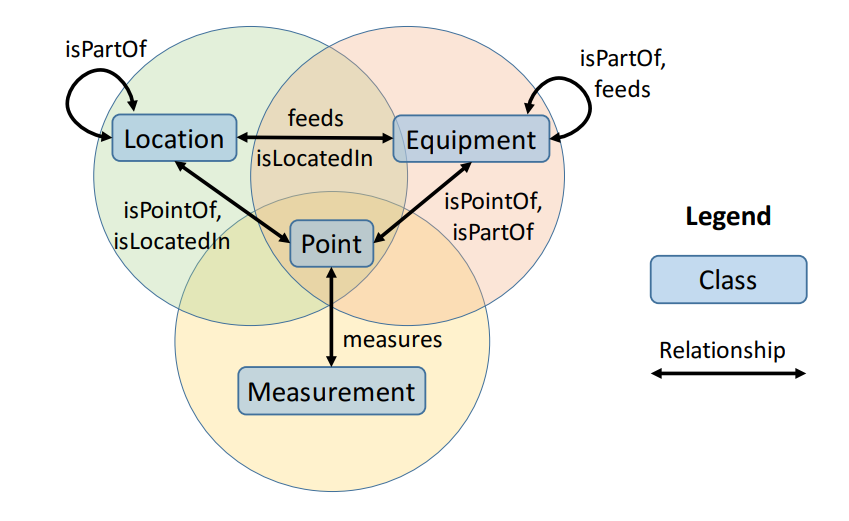
\includegraphics[width=0.7\textwidth]{Images/Brick.png}
    \caption{\textbf{Information concepts in Brick and their relationship
to a data point}~\cite{Balaji2016Brick}}
    \label{fig:Brick}
\end{figure}

Brick's key strengths include its clarity, expressiveness, and
demonstrated portability. In a validation involving six heterogeneous
buildings totaling approximately 630,000 ft\textsuperscript{2} and about
17,700 BMS data points, Brick achieved mapping coverage of around
98\% of the metadata and supported eight representative applications—
such as occupancy analytics, fault detection, demand response, and
energy apportionment—without modification~\cite{Balaji2016Brick}.
These results highlight how a compact, orthogonal schema can
significantly reduce integration costs and enable cross-site reuse of
analytics and control logic.

However, Brick also has limitations when considered in the context of
transportation systems. Its focus on static subsystems within buildings
means it lacks native constructs to represent \emph{temporal events}
(e.g., EV charging sessions), \emph{mobile entities} (e.g., vehicles), or
domain-specific regulatory and forecasting aspects. For example, a
recent evaluation of semantic technologies in building energy
flexibility found that Brick could represent only about 16\% of EV
charging–related concepts, and entirely failed to capture regulatory
constraints or environmental forecast information.
Therefore, while Brick is effective in building-scale modeling, it must
be complemented with dynamic, context-aware frameworks such as
NGSI-LD for applications in EV charging infrastructure and smart
mobility systems.

In summary, Brick combined with RDF provides a powerful and
well-structured way to model static building metadata, making
equipment, sensors, and spaces machine-readable and portable across
sites. The use of RDF triples and SPARQL enables interoperability and
semantic reasoning that are essential for digital twin applications at the
building scale. Nevertheless, Brick is less suited to domains that require
continuous handling of dynamic, time-varying data and mobile entities,
such as transportation systems and EV charging infrastructures. These
scenarios demand data models capable of representing temporal events,
context updates, and cross-domain interactions in real time. 

\section{Web of Things (WoT)}

The WoT initiative began around 2014 within the World Wide Web Consortium (W3C) Interest Group
and was formalized in the WoT Working Group, with the first
recommendations—covering the WoT Architecture and the Thing
Description—published in 2020~\cite{W3CWOT2020}.W3C is an international standards
organization founded in the United States in 1994 but with a
globally distributed membership and governance.

At its core is the \emph{Thing Description} (TD), a machine-readable
document based on JSON-LD that specifies the metadata, properties,
actions, and events of a device~\cite{W3CWOT2020}. A TD serves as a
semantic contract between a device (the “Thing”) and applications,
allowing developers to interact with devices through uniform APIs
regardless of vendor-specific protocols.

\begin{figure}[ht]
    \centering
    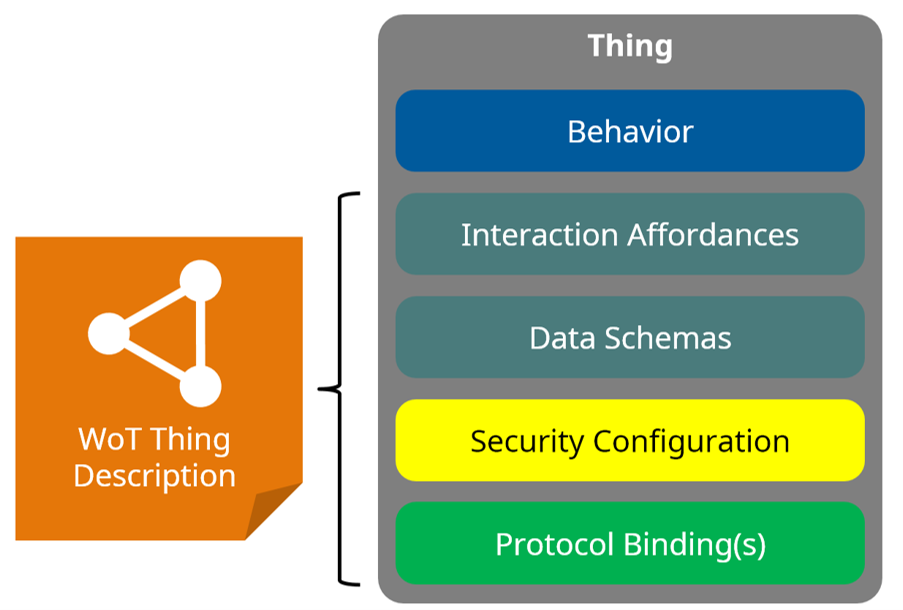
\includegraphics[width=0.3\textwidth]{Images/td.png}
    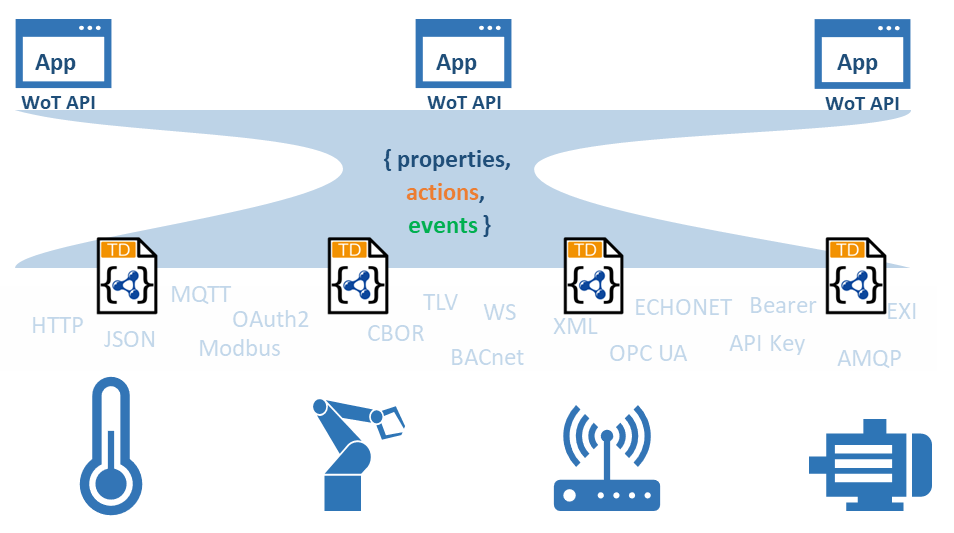
\includegraphics[width=0.35\textwidth]{Images/wot-mappings.png}
    \caption{\textbf{IoT Metadata in TD (left) and WoT mappings (right)} \\In general, WoT is a protocol agnostic approach and provides a common mechanism to define how specific protocols such as MQTT, HTTP, CoAP or Modbus can be mapped to the WoT's interaction properties-action-event abstraction.~\cite{W3CWOT2020}}
    \label{fig:image2}
\end{figure}


The strengths of WoT lie in its ability to provide a lightweight,
technology-agnostic abstraction for devices. By describing
functionalities in JSON-LD, WoT enables semantic interoperability
between devices that expose different protocols (e.g., HTTP, CoAP,
MQTT). This abstraction facilitates integration of IoT devices into
larger ecosystems, allowing web applications, gateways, and digital
twin platforms to discover and use device capabilities in a consistent
way. The WoT standard is also modular, supporting security,
binding templates, and scripting APIs, which together ease the
deployment of scalable IoT systems.

Despite these advantages, WoT also has limitations when applied to
transportation and EV charging infrastructure. WoT focuses on the
device level—standardizing access to sensors and actuators—but it
does not by itself provide higher-level semantics for systems such as
charging networks, mobility services, or energy markets. As a result,
WoT alone cannot capture domain-specific relationships (e.g., vehicle
arrival events linked to charging tariffs, or the coordination between
multiple charging stations). In practice, WoT is most effective when
used in combination with higher-level frameworks which can
forming a layered approach to interoperability in smart transport
systems.

\section{FIWARE and NGSI-LD}

FIWARE is an open-source platform initiative launched in 2011 under
the European Union’s Seventh Framework Programme (FP7), initially
supported by the European Commission and a consortium of European
companies and research organizations. It is now managed by the
FIWARE Foundation, a non-profit association based in Berlin, Germany,
which coordinates global adoption of FIWARE technologies across smart
cities, energy, industry, and mobility. At the heart of FIWARE is the
\emph{Context Broker}, the core component that manages context
information about entities in the physical and digital world. The most
widely used implementation is the Orion Context Broker and its
NGSI-LD compliant extension Orion-LD.

The FIWARE Next Generation Service Interfaces (NGSI) define the
standard API for context management. NGSI-LD, standardized by ETSI
(European Telecommunications Standards Institute) in 2019, extends
earlier NGSI versions by adopting linked-data principles and JSON-LD
serialization~\cite{ETSI2019NGSILD}. It provides an entity–property–
relationship model that is semantically interoperable and aligned with
semantic web technologies. Each NGSI-LD entity can represent a
real-world object (e.g., an EV charging station), its properties (e.g.,
capacity, current load), and its relationships (e.g., connected to a power
grid or located in a district). The Context Broker exposes these entities
via a publish–subscribe API, allowing real-time updates and
notifications.

\begin{figure}[ht]
    \centering
    
\includegraphics[width=0.7\textwidth]{Images/NGSI-LD-Architecture-Interactions.svg.png}
    \caption{\textbf{NGSI-LD Architecture Interactions} \\
    Context Consumer retrieves information through queries or subscriptions, Context Producer creates, updates, and deletes entity data, Context Broker serves as the primary access point that aggregates and returns data, Context Source stores data and announces available data types to the Registry Server, and Registry Server records data types from each Source to help the Broker discover required information.}
    \label{fig:orion}
\end{figure}

The strengths of FIWARE and NGSI-LD lie in their ability to handle
\emph{dynamic context} at scale. Through the Context Broker,
applications can subscribe to changes (e.g., a vehicle starting or
ending a charging session) and react immediately. This dynamic and
event-driven model is particularly advantageous in domains such as
transport and energy, where continuous synchronization with rapidly
changing environments is required. FIWARE also provides a broad
ecosystem of enablers—such as IoT agents, data processing
components, and dashboards—that simplify integration with IoT
devices and data platforms, facilitating large-scale deployments in
smart cities worldwide~\cite{Papadakis2022NGSI}.

Nevertheless, FIWARE and NGSI-LD also present challenges when
applied to transportation and EV charging infrastructure. While
NGSI-LD defines a generic model, it does not provide detailed domain
semantics for vehicles, tariffs, or multimodal transport flows. Developers
often rely on the \emph{Smart Data Models} initiative, jointly maintained
by the FIWARE Foundation, ETSI, and the Open \& Agile Smart Cities
(OASC) network, to obtain domain-specific schemas. Furthermore,
heterogeneous modeling practices across projects can hinder semantic
consistency, and complex cross-domain interactions (e.g., integrating
mobility services with energy markets) often require additional semantic
integration layers. 

\section{Internship Challenges and Contribution}

The analysis of related frameworks highlights that Brick, WoT, and
FIWARE each address different layers of interoperability.
Brick provides a static ontology for building metadata, WoT enables
device-level interoperability via standard Web interfaces, and
FIWARE offers a scalable framework for dynamic context
management in smart environments. Table~\ref{tab:comparison}
summarizes their origins, strengths, and limitations.

\begin{table}[htb]
\centering
\caption{Comparison of FIWARE, Brick, and WoT}
\label{tab:comparison}
\renewcommand{\arraystretch}{1.3} % 增加行间距
\begin{tabular}{|>{\raggedright\arraybackslash}p{2.8cm}|>{\raggedright\arraybackslash}p{4cm}|>{\raggedright\arraybackslash}p{4cm}|>{\raggedright\arraybackslash}p{4cm}|}
\hline
\textbf{Aspect} & \textbf{FIWARE} & \textbf{Brick} & \textbf{WoT} \\ 
\hline\hline
\textbf{Main focus} & 
Dynamic context management through Context Broker and NGSI-LD API & 
Semantic ontology framework for building metadata and relationships & 
Device interoperability via Web standards and protocols \\ 
\hline
\textbf{Modeling method} & 
NGSI-LD (Linked Data with JSON-LD serialization) & 
RDF + OWL ontology with SPARQL queries & 
Thing Description using JSON-LD and Web APIs \\ 
\hline
\textbf{Pros} & 
\begin{itemize}[leftmargin=*,nosep,after=\strut]
\item Real-time context updates
\item Subscription mechanisms
\item Cross-domain interoperability
\item Scalable REST APIs
\end{itemize} & 
\begin{itemize}[leftmargin=*,nosep,after=\strut]
\item Unified building semantics
\item Strong reasoning capabilities
\item Rich relationship modeling
\item Standardized vocabulary
\end{itemize} & 
\begin{itemize}[leftmargin=*,nosep,after=\strut]
\item Protocol-agnostic access
\item Standardized APIs
\item Web integration
\item Device abstraction
\end{itemize} \\ 
\hline
\textbf{Cons} & 
\begin{itemize}[leftmargin=*,nosep,after=\strut]
\item Limited domain ontologies
\item Depends on Smart Data Models
\item Device-level control constraints
\end{itemize} & 
\begin{itemize}[leftmargin=*,nosep,after=\strut]
\item Weak dynamic data handling
\item Limited temporal modeling
\item Mainly static metadata focus
\end{itemize} & 
\begin{itemize}[leftmargin=*,nosep,after=\strut]
\item Weak semantic reasoning
\item Limited complex system modeling
\item Primarily device-layer focus
\end{itemize} \\ 
\hline
\textbf{Organization} & 
FIWARE Foundation and ETSI & 
Brick Schema community & 
W3C \\ 
\hline
\end{tabular}
\end{table}

From this comparison, it becomes evident that while Brick and WoT
provide valuable capabilities, they are not sufficient for the specific
challenges of modeling and managing electric vehicle (EV) charging
infrastructure. Brick is too static to capture real-time charging events,
and WoT does not extend beyond device-level descriptions. In
contrast, FIWARE and its NGSI-LD standard are designed for
real-time, cross-domain interoperability and have already been
adopted in numerous European smart city and energy projects.

Given that this research is funded within the European context, FIWARE is a natural choice as it is an EU
initiative, standardized by ETSI, and actively supported by the FIWARE
Foundation. Beyond alignment with funding priorities, FIWARE is also
technically best suited for the EV charging scenario, as it provides the
necessary dynamic context management, integration of IoT data, and
publish–subscribe mechanisms required for real-time infrastructure
simulation.

Although FIWARE has proven effective
for smart city applications, some \textbf{challenges} remain. Its modeling focus is typically on the
city-wide or district scale (e.g., mobility services, energy demand). As such, the standard provides limited
support for station-level modeling that captures the detailed behavior
of individual EV charging station. This gap is critical, since station
operations involve specific characteristics such as connector types,
charging session dynamics, user behavior, and local grid interactions
that cannot be fully expressed through generic NGSI-LD entities.
Bridging this gap requires extending FIWARE-based models with
domain-specific concepts that can describe charging stations with
sufficient granularity. Without such refinements, digital twins built on
FIWARE risk losing fidelity at the level most relevant to operational
optimization.

This internship \textbf{contributes} to addressing the above challenges by:
\begin{itemize}
  \item Extending FIWARE from its traditional smart city
  scope to the \emph{charging station level}, enriching the model with
  entities and attributes that capture the operational details of EVSEs
  (Electric Vehicle Supply Equipment).
  \item Developing NGSI-LD compliant data models based on \emph{real
  data} collected from the E4C campus, ensuring that the digital twin
  framework reflects actual charging patterns, station utilization, and
  grid impacts.
  \item Implementing these models within the FIWARE ecosystem,
  centered on the Orion-LD Context Broker, and integrating them with
  supporting components for storage, monitoring, and simulation.
  \item Demonstrating how the refined FIWARE-based digital twin can
  provide actionable insights at the station level, supporting deployment
  strategies, demand forecasting, and operational optimization.
  \item Showing that the proposed approach is \emph{scalable and
  generalizable}, as the methodology applied to the E4C campus can
  be transferred to other campuses, districts, or urban areas to enable
  more detailed and interoperable EV charging infrastructure modeling.
\end{itemize}






% \section{Listes et tableaux}

% \textbf{Insérer une liste~:}
% \begin{itemize}
%     \item Premier niveau
%     \begin{itemize}
%         \item[(i)] Deuxième niveau
%         \item[(ii)] Un autre élément au deuxième niveau
%     \end{itemize}
%     \item Un autre élément au premier niveau
%         \begin{itemize}
%         \item[(a)] Deuxième niveau
%         \item[(b)] Un autre élément au deuxième niveau
%     \end{itemize}
% \end{itemize}
% \bigskip

% \textbf{Insérer un tableau simple~:} 
% \begin{table}[H]
%     \centering
%     \begin{tabular}{|c|c|c|c|c|c|c|c|c|c|}
%         \hline
%         A & B & C & D & E & F & G & H & I & \dots \\
%         \hline
%         1 & 2 & 3 & 4 & 5 & 6 & 7 & 8 & 9 & \dots\\
%         10 & 11 & 12 & 13 & 14 & 15 & 16 & 17 & 18 & \dots \\
%         \hline
%     \end{tabular}
%     \caption{\textbf{Titre.} \lipsum[1][1-3]}
%     \label{tab:table-label}
% \end{table}

% \textbf{Autre style de tableau~:} 
% \begin{table}[H]
%     \centering
%     \begin{tabular}{c c c c c}
%         \hline
%         \textbf{Col1} & \textbf{Col2} & \textbf{Col3} & \textbf{Col4} & \textbf{Col5} \\
%         \hline
%         1 & 2 & 3 & 4 & 5 \\
%         1 & 2 & 3 & 4 & 5 \\
%         \hline
%     \end{tabular}
%     \caption{\textbf{Titre.} \lipsum[1][1-3]}
%     \label{tab:table-label}
% \end{table}


% \section{Insertion de code Python}
% \textbf{Insérer du code en \textit{inline}~:} \texttt{print("Hello, World!")}.\\


% \textbf{Insérer du code en \textit{inline} avec coloration syntaxique~:} \mintinline{python}{print("Hello, World!")}.\\

% \textbf{Insérer du code en bloc avec coloration syntaxique~:} 
% \begin{minted}[bgcolor=codebg,fontsize=\small,frame=lines,linenos]{python}
% def factorial(n):
%     if n == 0:
%         return 1
%     else:
%         return n * factorial(n - 1)

% # Example usage
% print(factorial(5))  # Output: 120
% \end{minted}



% \section{Expressions mathématiques}
% \subsection{Théorèmes, propositions, définitions, lemmes, demonstrations...}

% \begin{theorem}
%     \lipsum[1][1-4]
% \end{theorem}

% \begin{proof}
%     \lipsum[1][1-4]
% \end{proof}

% \begin{proposition}
%     \lipsum[1][1-4]
% \end{proposition}

% \begin{definition}
%     \lipsum[1][1-4]
% \end{definition}

% \begin{remark}
%     \lipsum[1][1-4]
% \end{remark}

% \begin{lemma}
%     \lipsum[1][1-4]
% \end{lemma}


% \subsection{Equations et calculs sur plusieurs lignes}

% \subsubsection*{Une simple équation}
% \begin{equation}
%     e = mc^2
% \end{equation}

% \subsubsection*{Une équation sur plusieurs lignes}
% \begin{equation}
%     \begin{split}
%         \mathbb{E}(aX + Y) &= \mathbb{E}(aX) + Y\\
%                            &= a\mathbb{E}(X) + Y
%     \end{split}
% \end{equation}

% \subsubsection*{Une équation avec plusieurs cas}
% \begin{equation}
%     u_n =
%     \begin{cases}
%         1 \text{ if } n\equiv0 \mod 2\\
%         0 \text{ if } n\equiv1 \mod 2 \\
%     \end{cases}
% \end{equation}

% \subsubsection*{Insérer une série de calculs}
% \begin{align*}
%     x &= 0.999\ldots \\
%     10x &= 9.999\ldots \\
%     10x - x &= 9.999\ldots - 0.999\ldots \\
%     9x &= 9 \\
%     x &= 1 \\
%     0.999\ldots &= 1
% \end{align*}

% \subsection{Utilisation du glossaire}

% \newglossaryentry{esperance}{
%     name=espérance,
%     description={Valeur moyenne théorique d'une variable aléatoire}
% }


% Référence au glossaire : \gls{esperance}.  




